\section{机器阅读理解任务概述}

%\footnotetext[1]{\url{www.cnn.com}}\label{1}\vspace{-10pt}
机器阅读理解(MRC)任务是为了使得计算机具有对自然语言文本理解的能力,像人类一样阅读并且理解一篇文章。
MRC可以用一个三元组$<D,Q,A>$来描述,其中$D$代表文章(Document)\footnote{本文中文章(Document)和段落(Passage)是同样的概念},$Q$表示问题(Question),$A$表示答案(Answer),即
给定一篇文章$D$和一些与文章$D$相关的问题$Q$,
要求模型通过阅读$D$之后给出$Q$的正确答案$A$,即建模给定$D$和$Q$的条件下预测$A$的概率:$P(A|D,Q)$
。

近年来MRC任务越来越复杂,具体的体现就是数据集越来越具有挑战性。对于早期的填空型任务,模型仅仅需要阅读一篇文章,甚至只需某个相关的上下文句子即可正确的填写出问题中的单词。经过近几年的MRC领域的快速发展,目前已经有很多数据集既需要模型从多篇文章中多步推理又要同时给出不限于文章中单词的答案,任务的难度显著上升。
本文按照Chen\upcite{base}
提出的根据答案形式的不同将阅读理解任务概括为4类任务:填空式、多项选择式、抽取式和自由答案式。
%随着近年来MRC领域的发展出现了一些新兴的阅读理解任务如带有无答案问题的任务,对话形式的任务等,本文将机器阅读理解任务划分为yixia
下面对这四种类型任务分别进行叙述并介绍相关的数据集。



\subsection{填空式}
填空式阅读理解是指给定一篇文章$D$和一个与文章相关的问题$Q$,$Q$是通过删除
掉句子中某一个单词构成,要求模型根据$D$能够
正确的填写出$Q$缺失的单词$a$,且$a\in D$。填空型数据集的一个样例见表1。

CNN\&Daily Mail\upcite{CNNDailyMail}数据集是
由Google DeepMind和牛津大学发布于2015年,
这是第一个较大规模的完形填空型阅读理解型数据集。从CNN\footnote{www.cnn.com\label{cnn}}中收集93k篇文章,从
Daily Mail\footnote{www.dailymail.co.uk\label{daily mail}}上收集220k篇文章。删去句子中的一个命名实体单词,
以此作为问题,构建了(文章-问题-答案)的三元组形式的语料库作为填空式的阅读理解任务。

Hill等人\upcite{CBT}发布了(Children's Book Test,CBT)数据集,语料库来源于儿童读物(Gutenberg\footnote{https://www.gutenberg.org/\label{cbt}}工程)。每一篇文章是由20个连续的句子构成,删除第21个句子中的某个单词作为问题。与CNN\&Daily Mail的不同之处是删除的单词不局限于命名实体,还可能删除句子中的名词、动词和介词。

CLOTH\upcite{CLOTH}数据集是收集自中国中学生的英语考试试题中的完型填空题型。与之前的填空型数据集最大的不同是问题中删除的单词不像之前数据集的构建方式那样是由系统根据规则自动构建的,这样生成的问题往往没有目的性并且答案可能会出现歧义。
而是由教师为了测验学生英语水平而精心设计的,空白处位置的单词通常会考察学生的词汇、语法以及推理能力,因此CLOTH数据集相比于CNN\&Daily和CBT更具有挑战性。

%\begin{center}
\begin{table}[ht]
    %\centering
    %表格超出页边距用resizebox
    %\resizebox{\textwidth}{!}{
    \caption{CNN\&Daily Mail\upcite{CNNDailyMail}数据集的一个样例 \\ Table 1 An example of CNN\&Daily Mail dataset}
    %\vspace{5pt}

    \begin{tabular}{l p{15.0cm}<{\raggedright}}
        \toprule
        文章:&\tabincell{l}{What was supposed to be a fantasy sports car ride at Walt Disney World Speedway turned \\ 
                           deadly when a Lamborghini crashed into a guardrail. The crash took place Sunday at the \\ 
                           Exotic Driving Experience, which bills itself as a chance to drive your dream car on a race-\\ 
                           track. The Lamborghini’s passenger, 36-year-old Gary Terry of Davenport, Florida, died at \\ the
                           scene, Florida Highway Patrol said. The driver of the \textbf{Lamborghini}, 24-year-old Tavon \\ Watson
                            of Kissimmee, Florida, lost control of the vehicle, the Highway Patrol said. (...)} \\
        %\cmidrule(l){2-3}
        \midrule
        问题:&\tabincell{l}{Officials say the driver, 24-year-old Tavon Watson, lost control of a\_\_\_} \\
        %\cmidrule(l){2-3}
        \midrule
        答案:&Lamborghini \\
        \bottomrule
    \end{tabular}
    %}
    %\textbf{表1:CNN\& Daily Mail\upcite{Teaching Machines to Read and Comprehend}的一个样例}
\end{table}
%\end{center}

\subsection{多项选择式}
多项选择式这类问答任务是对于给定的文章$D$和问题$Q$以及多个
候选答案$A=\{A_1,A_2,\cdots,A_n\}$,
从中选择正确的答案,即建模概率:$P(A_i|D,Q)$,其中$A_i \in A$。
相关的数据集如MCTest\upcite{MCTest}和RACE\upcite{RACE}。多项选择型数据集的一个样例见表2。

MCTest是一个早期提出来的多项选择型数据集,问题形式为四选一。数据集收集自儿童故事语料库,类似这种基于故事文章的语料库
构建数据集的还有上面提到的CBT\upcite{CBT}。但是由于其规模比较小仅仅包含500篇故事文章很难利用神经网络模型来学习,因此MCTest通常用来作为验证集或测试集。

RACE\footnote{www.cs.cmu.edu/glail/data/race/\label{race}}数据集是从中
国中学生的英语考试题中的阅读理解题型
建立的数据集。共有将近28000篇文章以及100000个问题,
%答案并不是简单的限制于
%文章中的单词,而且答案和问题中单词可能
%从没有在文章中出现过,利用单词匹配方式并不能达到很好的效果。
这些问题和候选答案都是由出题专家生成的,更加的
接近真实世界的语义。
%RACE数据集中文章主题的覆盖度比其它的数据集更广泛,比如CNN\&Daily\upcite{CNNDailyMail}
%所有文章全都是来源于CNN新闻,SQuAD\upcite{SQuAD1}数据集所有的文章全都是来源于维基百科。
RACE数据集涵盖多个领域如新闻、故事、广告、传记等等,由于其类型的多样性因此可以更好的评估机器的阅读理解
能力。


\begin{table}[ht]
    %\centering
    %表格超出页边距用resizebox
    %\resizebox{\textwidth}{!}{
    \caption{RACE\upcite{RACE}数据集的一个样例 \\ Table 2 An example of RACE dataset}
    %\vspace{5pt}

    \begin{tabular}{l p{15.0cm}<{\raggedright}}
        \toprule
        文章:&\tabincell{l}{Runners in a relay race pass a stick in one direction. However, merchants passed silk, gold, \\ 
                           fruit, and glass along the Silk Road in more than one direction. They earned their living by \\ 
                           traveling the famous Silk Road. .. The Silk Road was made up of many routes, not one smo- \\oth 
                           path. They passed through what are now 18 countries. The routes crossed mountains and \\ deserts  
                           and had many dangers of hot sun, deep snow and even battles...}\\
        %\cmidrule(l){2-3}
        \midrule
        问题:&\tabincell{l}{The Silk Road became less important because\_\_\_} \\
        %\cmidrule(l){2-3}
        \midrule
        选项:& \tabincell{l}{A. it was made up of different routes \\
        B. silk trading became less popular \\
        \textbf{C. sea travel provided easier routes} \\
        D. people needed fewer foreign goods}\\
        %\cmidrule(l){2-3}
        \midrule
        答案:&C \\
        \bottomrule
    \end{tabular}
    %}
    %\textbf{表1:CNN\& Daily Mail\upcite{Teaching Machines to Read and Comprehend}的一个样例}
\end{table}

\subsection{抽取式}
这类阅读理解任务是MRC领域较为流行的研究方向,主要原因在于从数据集的构建、评测指标以及应用价值等角度上看抽取式阅读理解是最合适的。
给出文章$D$和问题$Q$,问题的答案是$D$中的一段连续的单词构成,
答案的长度不固定,可以表示为$P(A|D,Q)$,其中$A=\{t_i,t_{i+1},\cdots,t_{i+k}\}(1\leq i\leq i+k\leq n)$,$n$代表$D$中
单词的个数。片段选择型问答任务数据集较其它类型任务的数据集较多,常用的数据集如SQuAD\upcite{SQuAD1}、
NewsQA\upcite{NewsQA}、TriviaQA\upcite{TriviaQA}等。片段选择型的一个样例见表3。

SQuAD是MRC领域最为
广泛使用的数据集之一,它的提出极大地推动了MRC领域的发展。
数据集由众包工人根据维基百科上面的文章给出问题,答案来源于文章中某段连续的文本,长度并不固定。
SQuAD 1.1含有536篇文章,总计十万多个问题-答案对
。NewsQA数据集很类似于SQuAD,区别在于其文章来源于CNN新闻并且在NewsQA中某些问题
是没有答案的,这也使得后来Rajpurkar等人在SQuAD版本上又增加了五万个不可回答的问题构建了数据集SQuAD 2.0\upcite{SQuAD2}。对于这些带有不可回答问题的数据集,模型首先要清楚问题是否可以根据文章回答,在可回答的前提下给出答案,因此要求模型对文章的理解要更加的深刻。
%实验表明,那些在SQuAD数据集上效果很好的模型在SQuAD 2.0数据集上性能显著下降,这也说明了目前很多MRC模型都是基于浅层的语义匹配来寻找答案而不是真正的理解了文章。

TriviaQA数据集的构造方式不同于前面数据集的构造方式。之前的数据集都是给定文章后,由人工构造出与文章相关的问题和答案,但是现实世界中人们通常是先提出问题
然后搜寻相关的文章再找到答案。基于这一思想,Joshi等人首先从trivia上收集大量的问题-答案对,然后为每一个问题从网页上或者维基百科上搜索出相关的文章,这些文章就是答案的依据。最后构建出65万多个(问题-答案-文章)三元组,更重要的是这种由问题找文章的数据集构造方式使得问题和文章在句法和词汇上都有着较大的差异性,
这使得数据集难度更高。

尽管上面的数据集难度越来越高,但是它们整体上来说对模型的推理能力要求不高,主要原因在于回答这些数据集的问题往往只需要集中于某个句子的上下文或者在一篇段落上推理即可。为了提高模型的多步推理能力,
Yang等人\upcite{HotpotQA}发布了HotpotQA数据集,每一个问题对应多个段落,问题的答案往往需要在多个段落上逐步推理才能获得,类似的数据集还有WIKIHOP\upcite{WIKIHOP}等

\begin{table}[ht]
    %\centering
    %表格超出页边距用resizebox
    %\resizebox{\textwidth}{!}{
    \caption{SQuAD 1.1\upcite{SQuAD1}数据集的一个样例 \\ Table 3 An example of SQuAD 1.1 dataset}
    %\vspace{5pt}

    \begin{tabular}{l p{15.0cm}<{\raggedright}}
        \toprule
        文章:&\tabincell{l}{In 1870, Tesla moved to Karlovac, to \textbf{attend school at the Higher Real Gymnasium},\\ where
                            he was profoundly influenced by a math teacher Martin Sekulić. The classes were held\\ in German, 
                            as it was a school within the Austro-Hungarian Military Frontier. Tesla was able \\to perform int
                            egral calculus in his head, which prompted his teachers to believe that he was\\ cheating. He fini- shed a four-year term in three years, graduating in 1873. \\} \\
        %\cmidrule(l){2-3}
        \midrule
        问题:&Why did Tesla go to Karlovac? \\
        %\cmidrule(l){2-3}
        \midrule
        答案:&attend school at the Higher Real Gymnasium \\
        \bottomrule
    \end{tabular}
    %}
    %\textbf{表1:CNN\& Daily Mail\upcite{Teaching Machines to Read and Comprehend}的一个样例}
\end{table}
%\begin{multicols}{2}
\subsection{自由答案式}
简单的从文章中摘取一段文本可能并不能回答问题需要的答案,自由答案型阅读理解任务的答案是自由形式的
,不局限于文章中的某些单词,语法上往往是更加的灵活。
可以表示为$P(A|D,Q)$,其中$A\subseteq D$或$A\nsubseteq D$。
从文章中概括提炼出问题的答案也是更加的符合人类的阅读方式的,基于这些原因,自由回答式问答的数据集
也因此公布出来并且受到广泛的关注,
相关的数据集如MS MARCO\upcite{MSmarco}、DuReader\upcite{DuReader}和NarrativeQA\upcite{NarrativeQA},自由答案型数据集的一个样例见表4。

MS MARCO是由微软通过在必应搜索引擎的日志上收集用户
提出的问题,对于文本段落是来源于必应搜索引擎的返回的搜索结果。具体的就是对于每一个问题,给出10个最相关的
查询结果的文本段落,然后由标注人员从这10个文本段落中找出那些与这个问题有
关的文本段落,人工的从这些选择出来的段落中
概括提炼出答案,同时对于选出来的段落要标记为$\text{is\_select=1}$,表示这个段落和答
案相关,从而可
以训练模型。如果不能从给出的10个段落中推理出答案,
那么这个问题就标记为不可回答的问题,同样要保留在数据集中,
目的就是让模型能够判别出问题是否可以回答。

DuReader是中文MRC数据集,类似于MS MARCO数据集的构造方式,问题和文章取自百度搜索和百度知道。
答案同样是人工生成的,一个问题会给出5个相应的文本段落,很多问题需要推理多篇文章段落才能得到答案,甚至一些问题存在多个答案。
MS MARCO和DuReader数据集的问题都是收集自搜索引擎中用户提出的问题,因此这两个数据集也更加的贴近真实场景。

Kovcisky等人认为现在MRC领域大部分数据集的问题过于肤浅,而且答案往往只关注上下文信息,因此很多问题仅仅通过浅层的模式匹配
就可以找到答案,他们发布的NarrativeQA数据集,收集自小说和电影剧本,要求模型在理解整部小说或剧本的前提下才能回答问题,要求模型需要有更强的理解能力和推理能力。


%\vspace{15\baselineskip}

\begin{table}[ht]
    %\centering
    %表格超出页边距用resizebox
    %\resizebox{\textwidth}{!}{
    \caption{MS MARCO\upcite{MSmarco}数据集的一个样例 \\ Table 4 An example of MS MARCO dataset}
    %\vspace{5pt}
	\centering%p{15.5cm}<{\raggedright}
    \begin{tabular}{l p{15.0cm}<{\raggedright}}
        \toprule
        文章1:&\tabincell{l}{Rachel Carson’s essay on The Obligation to Endure,is a very convincing argument about the \\
        harmful uses of chemical, pesticides, herbicides and fertilizers
        on the environment.} \\

        $.......$ \\
        文章5:&\tabincell{l}{Carson believes that as man tries to eliminate unwanted insects and weeds; however he is 
        act-\\ually causing more problems by polluting the environmen with, 
        for example, DDT and harm-\\ing living things}\\
        %\cmidrule(l){2-3}
        $.......$ \\
        文章10:&\tabincell{l}{Carson subtly defers her writing in just the right
        writing for it to not be subject to an induc-\\tion run
        rampant style which grabs the readers interest without
        biasing the whole article.}\\
        \hline
        问题:&Why did Rachel Carson write an obligation to endure? \\
        %\cmidrule(l){2-3}
        \midrule
        答案:&\tabincell{l}{Rachel Carson writes The Obligation to Endure
        because believes that 
        as man tries to elimin-\\ate 
        unwanted insects and weeds; however he is actually
        causing more problems by polluting \\ the environment.} \\
        \bottomrule
    \end{tabular}
    %}
    %\textbf{表1:CNN\& Daily Mail\upcite{Teaching Machines to Read and Comprehend}的一个样例}
\end{table}

%\subsection{对话型问答}
%虽然本节介绍的对话型任务按照答案形式上划分仍然可以划分到那四种类型里面,但是由于对话型问答任务与其它任务在数据集构造方式以及任务形式上有较大不同,因此本节单独列出对话型问答任务。
%除了按照答案形式上划分还可以根据文章类型划分,如单段落型阅读理解还是多段落型阅读理解。
%%
%%
%%根据问答形式划分,比如上面所介绍的所有数据集都属于单轮对话式问答,
%%即文章所对应的多个问题之间没有联系,每一个问题都是互相独立的。这并不符合
%%现实世界中人与人之间的对话交流,人们是通过多轮对话形式来交流的,每一轮的问题和答案都会影响后面的问答情况。
%然而无论是单段落型阅读理解还是多段落型阅读理解,它们都属于单轮对话问答,即问答的形式只有一轮,后面的问题与前面的问题和答案无关,每一个问题都是互相独立的。
%而在现实世界中人们是通过多轮对话形式来交流的,每一轮的问题和答案都会影响后面的问答情况。
%所以对话型任务来讲,在回答当前轮的问题时不仅需要考虑文章还需要考虑前几轮的问题和答案。
%具体可以表示为:给定$Q_i,D,{Q_{i-1},\cdots,Q_{i-k}},{A_{i-1},\cdots,A_{i-k}}$要求模型给出$A_{i}$。其中$Q_i,A_i$表示第$i$轮的问题和答案,$D$表示文章,$Q_{i-1},\cdots,Q_{i-k}$和$A_{i-1},\cdots,A_{i-k}$分别表示前$k$轮的问题和答案。即建模概率:
%\begin{equation}
%P(A_i|D,Q_i,Q_{i-1},\cdots,Q_{i-k},A_{i-1},\cdots,A_{i-k})
%\end{equation}
%
%目前典型的对话型问答数据集有CoQA\cite{CoQA}以及QuAC\cite{QuAC}。
%不同之处在于CoQA数据集的答案形式较为简单,类似于SQuAD 1.1\cite{SQuAD1},但是包含有yes/no以及unknown问题,其中unknown代表不可回答问题,此外还有一定比例的问题是自由答案形式。而QuAC数据集的构造过程中提问者没有看过文章而仅仅了解文章的标题,由回答者根据文章的内容选择出文章的一段文本作为答案,这种数据集构造形式类似于用户在搜素引擎中输入问题查找答案,目的是减少问题和文本之间的依赖,使得模型尽量避免通过浅层的匹配方式获得答案。
%对话型阅读理解数据集的一个样例见表5.其中每一个$R_i$代表答案依据,提供给模型训练。
%
%\begin{table}
%	\centering
%	\caption{对话型问答的一个样例,取自CoQA\cite{CoQA}}
%	\vspace{10pt}
%	\resizebox{\textwidth}{!}{\begin{tabular}{l p{15.5cm}<{\raggedright}}
%			\toprule
%			\multirow{3}{*}{文章}&Jessica went to sit in her rocking chair. Today was her birthday and she was turning 80. Her granddaughter Annie was coming over in the afternoon and Jessica was very excited to see her. Her daughter Melanie and Melanie's husband Josh were coming as well.\\
%			\cmidrule{2-2}
%			\multirow{3}{*}{第一轮}&$Q_1$: Who had a birthday? \\
%			&$A_1$: Jessica \\
%			&$R_1$: Jessica went to sit in her rocking chair. Today was her birthday and she was turning 80. \\
%			\cmidrule{2-2}
%			\multirow{3}{*}{第二轮}&$Q_2$: How old would \textbf{she} be? \\
%			&$A_2$: 80 \\
%			&$R_2$: she was turning 80. \\
%			\cmidrule{2-2}
%			\multirow{3}{*}{第三轮}&$Q_3$: Did \textbf{she} plan to have any visitors? \\
%			&$A_3$: Yes \\
%			&$R_3$: Her granddaughter Annie was coming over \\
%			\cmidrule{2-2}
%			\multirow{3}{*}{第四轮}&$Q_4$: \textbf{How many?} \\
%			&$A_4$: Three \\
%			&$R_4$: Her granddaughter Annie was coming over in the afternoon and Jessica was very excited to see her. Her daughter Melanie and Melanie's husband Josh were coming as well. \\
%			\cmidrule{2-2}
%			\multirow{3}{*}{第五轮}&$Q_5$: \textbf{Who?} \\
%			&$A_5$: Annie, Melanie and Josh \\
%			&$R_5$: Her granddaughter Annie was coming over in the afternoon and Jessica was very excited to see her. Her daughter Melanie and Melanie's husband Josh were coming as well. \\
%			\toprule  
%	\end{tabular}}
%\end{table}

%\begin{figure}[ht]
%	\centering
%	\caption{CoQA\upcite{CoQA}数据集的一个样例}
%	\vspace{10pt}
%	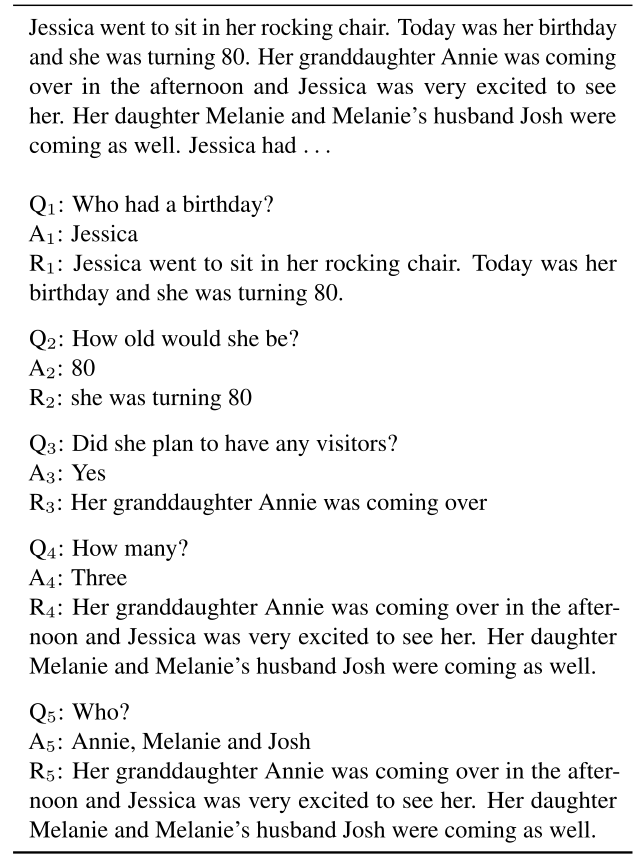
\includegraphics[width=8cm,height=10cm]{coqa.png}
%\end{figure}
\subsection{评估方法}
对于不同的MRC任务有不同的评估指标。
对于填空型任务与多项选择型任务都是属于客观题型,用准确率就可以衡量模型的性能。
例如对于测试集合中的所有问题$Q=\{Q_1,$$Q_2,\cdots,Q_m\}$,其中$m$代表问题的个数。如果模型预测出来的
$m$个答案中有$n$个是正确的,那么模型的准确率是$n/m$。

片段选择型任务属于半客观题型,通常用精确匹配EM(Exact Match)和F1分数来评估模型。
精确匹配EM评估指标可以看做是准确率的扩展,就片段选择型任务来讲,EM要求
预测出来的所有单词要和标准答案
的所有单词要完全一致,EM值才为1,否则为0。

F1值的计算方式是一种模糊匹配,它是精确率和召回率
之间的调和平均数。精确率是指模型预测的答案中有多大比例的单词是标准答案中的单词。
召回率是指标准答案中的单词有多大比例在预测答案中出现。


对于自由答案型任务由于其答案形式不固定,一般采用单词水平的匹配率作为评分标准,常用标准用
ROUGE-L\upcite{Rouge}和BLEU\upcite{BLEU}。ROUGE-L用来计算标准答案和预测答案的最长公共子序列(Longest Common Subsequence,LCS),BLEU最初用于评估翻译性能,在应用到MRC任务上主要
用来衡量预测答案和真实答案之间的相似性。表5列举了本章介绍的所有数据集。


%\subsubsection{ROUGE}
%ROUGE\upcite{ROUGE}(Recall-Oriented Understudy for Gisting Evaluation)最初是用来
%评估生成文本摘要的一种方法,因为可以ROUGE的计算机制
%来评估MRC领域中自由答案型任务。ROUGE的评分有多种,在MRC领域较为常用的是ROUGE-L,
%ROUGE-L用来计算标准答案和预测答案的最长公共子序列(Longest Common Subsequence,LCS),
%ROUGE-L的计算
%公式如下:
%\begin{gather}
%    R_{LCS}=\displaystyle\frac{LCS(X,Y)}{m} \notag \\
%    P_{LCS}=\displaystyle\frac{LCS(X,Y)}{n} \\
%    F_{LCS}=\displaystyle\frac{{(1+\beta)}^2R_{LCS}P_{LCS}}{R_{LCS}+\beta^2P_{LCS}} \notag
%\end{gather}
%其中$LCS(X,Y)$表示标准答案与预测答案之间的最长公共子序列,
%$m$和$n$分别代表标准答案和预测答案中单词的个数,$\beta$是ROUGE-L的的参数,
%用来控制精确率和召回率的重要程度。

%\subsection{小结}
%本章介绍了MRC任务的定义以及根据答案类型的不同划分四种任务并且介绍了每一个任务的形式以及相关的数据集
%,同时简述了每一个任务下衡量模型性能所用的评估指标。
%下表5从数据集来源及规模,文章、问题以及答案的类型角度上对比了本章所介绍的所有数据集(其中QuAC和CoQA两个数据集细节见\ref{cmrc}节)。可以看到,MRC任务从最简单的填空型任务,逐步过渡到复杂的片段选择型任务,最后到更复杂的需要从多段落进行多步推理或者对话形式的任务。正是这些越来越具有挑战性的数据集的发布,极大的推动了MRC领域的发展。
\begin{table}[ht]
	\centering
	\caption{MRC常用数据集对比,Acc代表准确率 \\ Table 5 Comparison of common dataset in MRC}
	%\vspace{5pt}
	\resizebox{\textwidth}{!}{
		\begin{tabular}{l c c c c c c}
			\toprule
			数据集&发布时间&文章来源&文章类型&问题特征&答案类型&评估指标 \\
			\midrule
			CNN\&Daily Mail\upcite{CNNDailyMail}&2015&新闻&单段落型&自动生成&填空式&Acc \\
			\midrule
			CBT\upcite{CBT}&2015&儿童读物&单段落型&自动生成&填空式&Acc \\
			\midrule
			CLOTH\upcite{CLOTH}&2016&英语考试&单段落型&人工生成&填空式&Acc \\
			\midrule
			MCTest\upcite{MCTest}&2013&儿童读物&单段落型&众包生成&多项选择式&Acc \\
			\midrule
			RACE\upcite{RACE}&2018&英语考试&单段落型&人工生成&多项选择式&Acc\\
			\midrule
			SQuAD\upcite{SQuAD1}&2016&维基百科&单段落型&众包生成&抽取式&EM/F1\\
			\midrule
			TriviaQA\upcite{TriviaQA}&2017&网页搜索&多段落型&收集于网站上的问题-答案对&抽取式&EM/F1\\
			\midrule
			SQuAD 2.0\upcite{SQuAD2}&2018&维基百科&单段落型&新增无答案问题&抽取式&EM/F1\\
			\midrule
			NewsQA\upcite{NewsQA}&2017&新闻&单段落型&众包生成,包含无答案问题&抽取式&EM/F1\\
			\midrule
			HotpotQA\upcite{HotpotQA}&2018&维基百科&多段落型&众包生成,需多步推理&抽取式&EM/F1\\
			\midrule
			WIKIHOP\upcite{WIKIHOP}&2018&维基百科&多段落型&自动生成,需多步推理&抽取式&EM/F1 \\
			\midrule
			MS MARCO\upcite{MSmarco}&2016&搜素引擎&多段落型&收集于搜索引擎&自由答案式&ROUGE-L/BLEU\\
			\midrule
			DuReader\upcite{DuReader}&2018&搜索引擎&多段落型&收集于搜索引擎&自由答案式&ROUGE-L/BLEU\\
			\midrule
			NarrativeQA\upcite{NarrativeQA}&2017&小说和电影剧本&多段落型&众包生成&自由答案式&ROUGE-L/BLEU\\
%			\midrule
%			CoQA\upcite{CoQA}&2018&维基百科/127K&单段落型&提问者和回答者以对话形式生成问题和答案&自由答案型\\
%			\midrule
%			QuAC\upcite{QuAC}&2018&维基百科/100K&单段落型&类似于CoQA,不过文章对于提问者不可见&片段选择型\\
			\bottomrule
		\end{tabular}
	}
\end{table}



